\documentclass{article}
\usepackage{amsmath}
\usepackage{mathtext}
\usepackage[T1,T2a]{fontenc}
\usepackage[utf8]{inputenc}
\usepackage[english, bulgarian, russian]{babel}
\usepackage{tikz}
\usepackage{longtable}
\usepackage{verbatim} 
\usepackage{multirow}
\usepackage{pgfplots}
\usepackage[export]{adjustbox}
\usepackage[left=2cm,right=2cm,
    top=2cm,bottom=2cm,bindingoffset=0cm]{geometry}

\begin{document}

\section{Элементарные частицы}

В этом пункте мы рассмотрим элементарные частицы стандартной модели обнаруженные и предсказаные.

Их можно условно разделить на три класса:

\subsection{Вещество}

\subsubsection{Кварки}

Кварки участвуют в сильных, слабых, электромагнитных и гравитационных взаимодействиях. Сильные взаимодействия (обмен глюоном) могут изменять цвет кварка, но не меняют его аромат. Слабые взаимодействия, наоборот, не меняют цвет, но могут менять аромат. Кварки имеют античастицы, обладающие такой же массой и обратным зарядом. Все кварки обладают спином 1/2.Необычные свойства сильного взаимодействия приводят к тому, что одиночный кварк не может удалиться на какое-либо существенное расстояние от других кварков, а значит, кварки не могут наблюдаться в свободном виде. Математический аппарат теории кварков основан на экспериментально подтверждённом предположении, что взаимодействия кварков инвариантны относительно группы изоспиновых преобразований SU(3)

\begin{center}
\begin{tabular}{|c|c|c|}
\hline
Символ кварка/антикварка (аромат)&Масса&заряд\\
\hline
u/\overline{u} & $1.5 \tilde 3$ & +2/3\\
\hline
d/\overline{d}&$4.79 \pm 0.07$&-1/3\\
\hline
c/\overline{c}&$1250 \pm 90$&+2/3\\
\hline
s/\overline{s}&$95 \pm 25$&-1/3\\
\hline
t/\overline{t}&$174340 \pm 790$&+2/3\\
\hline
b/\overline{b}&$4200 \pm 70$&-1/3\\
\hline
\end{tabular}
\end{center}

\subsubsection{Лептоны}

Лептоны не участвуют в сильном взаимодействии. Они также обладают античастицами с противоположным зарядом и такой же массой. Все лептоны обладают спином 1/2. Каждому заряженному лептону соответствует лёгкий нейтральный лептон — нейтрино. Ранее считалось, что каждое поколение лептонов обладает своим флейворным лептонным зарядом, — иными словами, лептон может возникнуть только вместе с антилептоном из своего поколения, так, чтобы разность количества лептонов и антилептонов каждого поколения в замкнутой системе была постоянной. Эта разность называется электронным, мюонным или тау-лептонным числом, в зависимости от рассматриваемого поколения. Лептонное число лептона равно +1, антилептона — −1. С открытием осцилляций нейтрино обнаружено, что это правило нарушается: электронное нейтрино может превратиться в мюонное или тау-нейтрино и т. д. Таким образом, флейворное лептонное число не сохраняется.

\begin{center}
\begin{tabular}{|c|c|c|}
\hline
Название&Заряд&Масса (МэВ)\\
\hline
Электрон&-1&0.511\\
\hline
Мюон&-1&105.66\\
\hline
Тау-лептон&-1&1776.99\\
\hline
Электронное нейтрино&0&$<2.2 \cdot 10^{-6}$\\
\hline
Мюонное нейтрино&0&<0.17\\
\hline
Тау-нейтрино&0&<15.5\\
\hline
\end{tabular}
\end{center}

\subsection{Переносчики взаимодействия}

Частицы переносчики четырех фунламентальных взаимодействий. 
\begin{center}
\begin{tabular}{|c|c|c|c|c|}
\hline
Название&Заряд (е)&Спин&Масса (ГэВ)&Переносимое взаимодействие\\
\hline
Фотон&0&1&0&Электромагнитное\\
\hline
$W^{\pm}$&$\pm 1$&1&80.4&Слабое взаимодействие\\
\hline
$Z^0$&0&1&91.2&Слабое взаимодействие\\
\hline
Глюон&0&1&0&Сильное взаимодействие\\
\hline
Бозон Хиггса&0&0&$\approx 125.09 \pm 0.24$&Инертная масса\\
\hline
Гравитон?&0&2&0&Гравитация\\
\hline
\end{tabular}
\end{center}

Гравитон является гипотетической частицей. Попытки расширить Стандартную модель гравитонами сталкиваются с серьёзными теоретическими сложностями в области высоких энергий (равных или превышающих планковскую энергию) из-за расходимостей квантовых эффектов. Решение этих вопросов было мотивом построения нескольких предложенных теорий квантовой гравитаци.

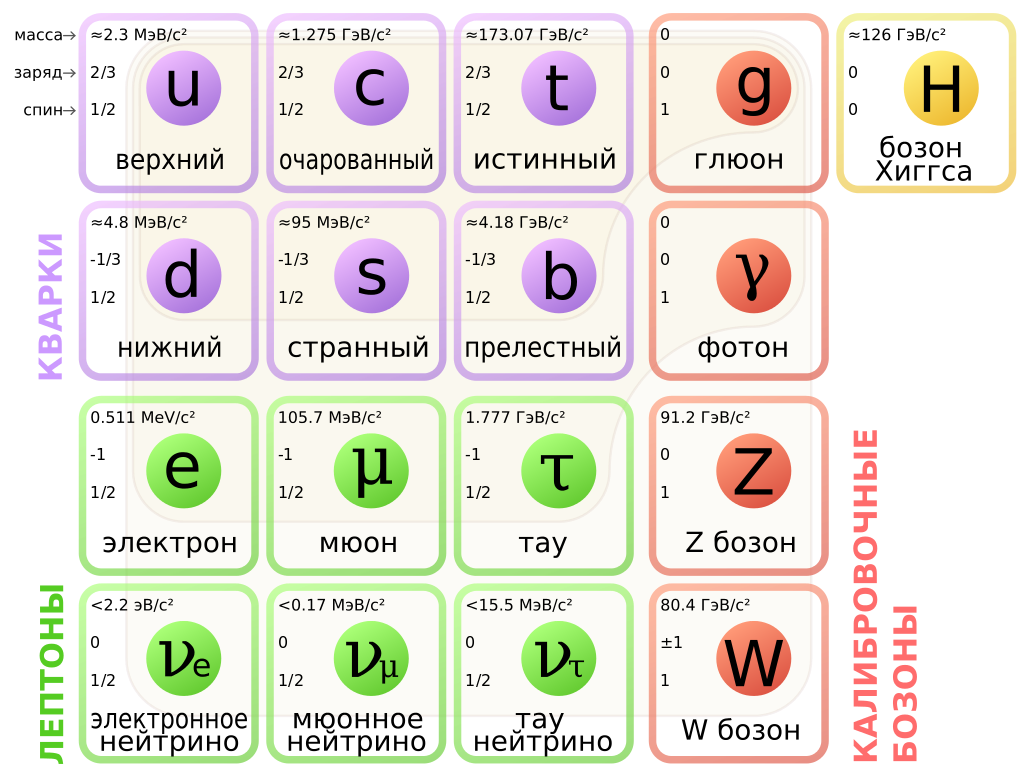
\includegraphics[width=1\textwidth]{basic_particles.png}


\end{document}